\documentclass[11pt,]{article}
\usepackage[left=1in,top=1in,right=1in,bottom=1in]{geometry}
\newcommand*{\authorfont}{\fontfamily{phv}\selectfont}



\usepackage[]{mathpazo}


  \usepackage[T1]{fontenc}
  \usepackage[utf8]{inputenc}

\usepackage{abstract}
\renewcommand{\abstractname}{}    % clear the title
\renewcommand{\absnamepos}{empty} % originally center

\renewenvironment{abstract}
 {{%
    \setlength{\leftmargin}{0mm}
    \setlength{\rightmargin}{\leftmargin}%
  }%
  \relax}
 {\endlist}

\makeatletter
\def\@maketitle{%
  \newpage
%  \null
%  \vskip 2em%
%  \begin{center}%
  \let \footnote \thanks
    {\fontsize{18}{20}\selectfont\raggedright  \setlength{\parindent}{0pt} \@title \par}%
}
%\fi
\makeatother




\setcounter{secnumdepth}{0}


\usepackage{graphicx,grffile}
\makeatletter
\def\maxwidth{\ifdim\Gin@nat@width>\linewidth\linewidth\else\Gin@nat@width\fi}
\def\maxheight{\ifdim\Gin@nat@height>\textheight\textheight\else\Gin@nat@height\fi}
\makeatother
% Scale images if necessary, so that they will not overflow the page
% margins by default, and it is still possible to overwrite the defaults
% using explicit options in \includegraphics[width, height, ...]{}
\setkeys{Gin}{width=\maxwidth,height=\maxheight,keepaspectratio}

\title{Lab 4: Vegetation transects \& ecosystem management \thanks{\textbf{Current version}: March , 2019}  }



\author{\Large BIO 3103, Baylor University\vspace{0.05in} \newline\normalsize\emph{}  }


\date{}

\usepackage{titlesec}

\titleformat*{\section}{\Large\bfseries}
\titleformat*{\subsection}{\normalsize\itshape}
\titleformat*{\subsubsection}{\normalsize\itshape}
\titleformat*{\paragraph}{\normalsize\itshape}
\titleformat*{\subparagraph}{\normalsize\itshape}





\newtheorem{hypothesis}{Hypothesis}
\usepackage{setspace}

\makeatletter
\@ifpackageloaded{hyperref}{}{%
\ifxetex
  \PassOptionsToPackage{hyphens}{url}\usepackage[setpagesize=false, % page size defined by xetex
              unicode=false, % unicode breaks when used with xetex
              xetex]{hyperref}
\else
  \PassOptionsToPackage{hyphens}{url}\usepackage[unicode=true]{hyperref}
\fi
}

\@ifpackageloaded{color}{
    \PassOptionsToPackage{usenames,dvipsnames}{color}
}{%
    \usepackage[usenames,dvipsnames]{color}
}
\makeatother
\hypersetup{breaklinks=true,
            bookmarks=true,
            pdfauthor={BIO 3103, Baylor University ()},
             pdfkeywords = {},  
            pdftitle={Lab 4: Vegetation transects \& ecosystem management},
            colorlinks=true,
            citecolor=blue,
            urlcolor=blue,
            linkcolor=magenta,
            pdfborder={0 0 0}}
\urlstyle{same}  % don't use monospace font for urls

% set default figure placement to htbp
\makeatletter
\def\fps@figure{htbp}
\setlength{\intextsep}{25pt}  % sets space after text/before float figure
\makeatother

\usepackage{multicol}
\usepackage{textcomp}
\usepackage{textgreek}
\usepackage{pdflscape}
\usepackage{float}
\usepackage{booktabs}
\usepackage{makecell}
\usepackage[table]{xcolor}
\usepackage{fixltx2e}
\usepackage{hyperref}
\usepackage{graphicx}


% add tightlist ----------
\providecommand{\tightlist}{%
\setlength{\itemsep}{0pt}\setlength{\parskip}{0pt}}

\begin{document}
	
% \pagenumbering{arabic}% resets `page` counter to 1 
%


% \maketitle

{% \usefont{T1}{pnc}{m}{n}
\setlength{\parindent}{0pt}
\thispagestyle{plain}
{\fontsize{18}{20}\selectfont\raggedright 
\maketitle  % title \par  

}

{
   \vskip 13.5pt\relax \normalsize\fontsize{11}{12} 
\textbf{\authorfont BIO 3103, Baylor University} \hskip 15pt \emph{\small }   

}

}




\noindent  \hypertarget{background-information}{%
\section{Background information}\label{background-information}}

Ecosystem management aims to preserve or restore ecosystems to promote
services or functions of natural environments that humans find
beneficial. Wetlands provide habitat for a wide range of organisms, help
mitigate flooding, and act as natural water filters by removing
nutrients, pollutants, and sediments. Managers frequently assess an
ecosystem by who lives there, which depends on our ability to accurately
quantify community structure. Valuable data can be collected just by
noting what organisms are there (also called presence/absence data), or
by noting how many of those organisms are there (also called abundance
data).

The LWWs has historically been strongly dominated by \emph{Typha}
(cattail). Although native to Texas, cattails are very aggressive and
frequently dominant wetlands to the exclusion of other species. To
counter this dominance tendency, managers have tried to increase the
diversity of the plant community in some areas of the LWWs by planting
other species {[}especially \emph{Schenoplectus} (bulrush) and
\emph{Pontederia} (pickerelweed){]}, or by hand-harvesting cattail out
of some areas in the hopes that other species will colonize the open
areas (Fig. 1).

\begin{figure}
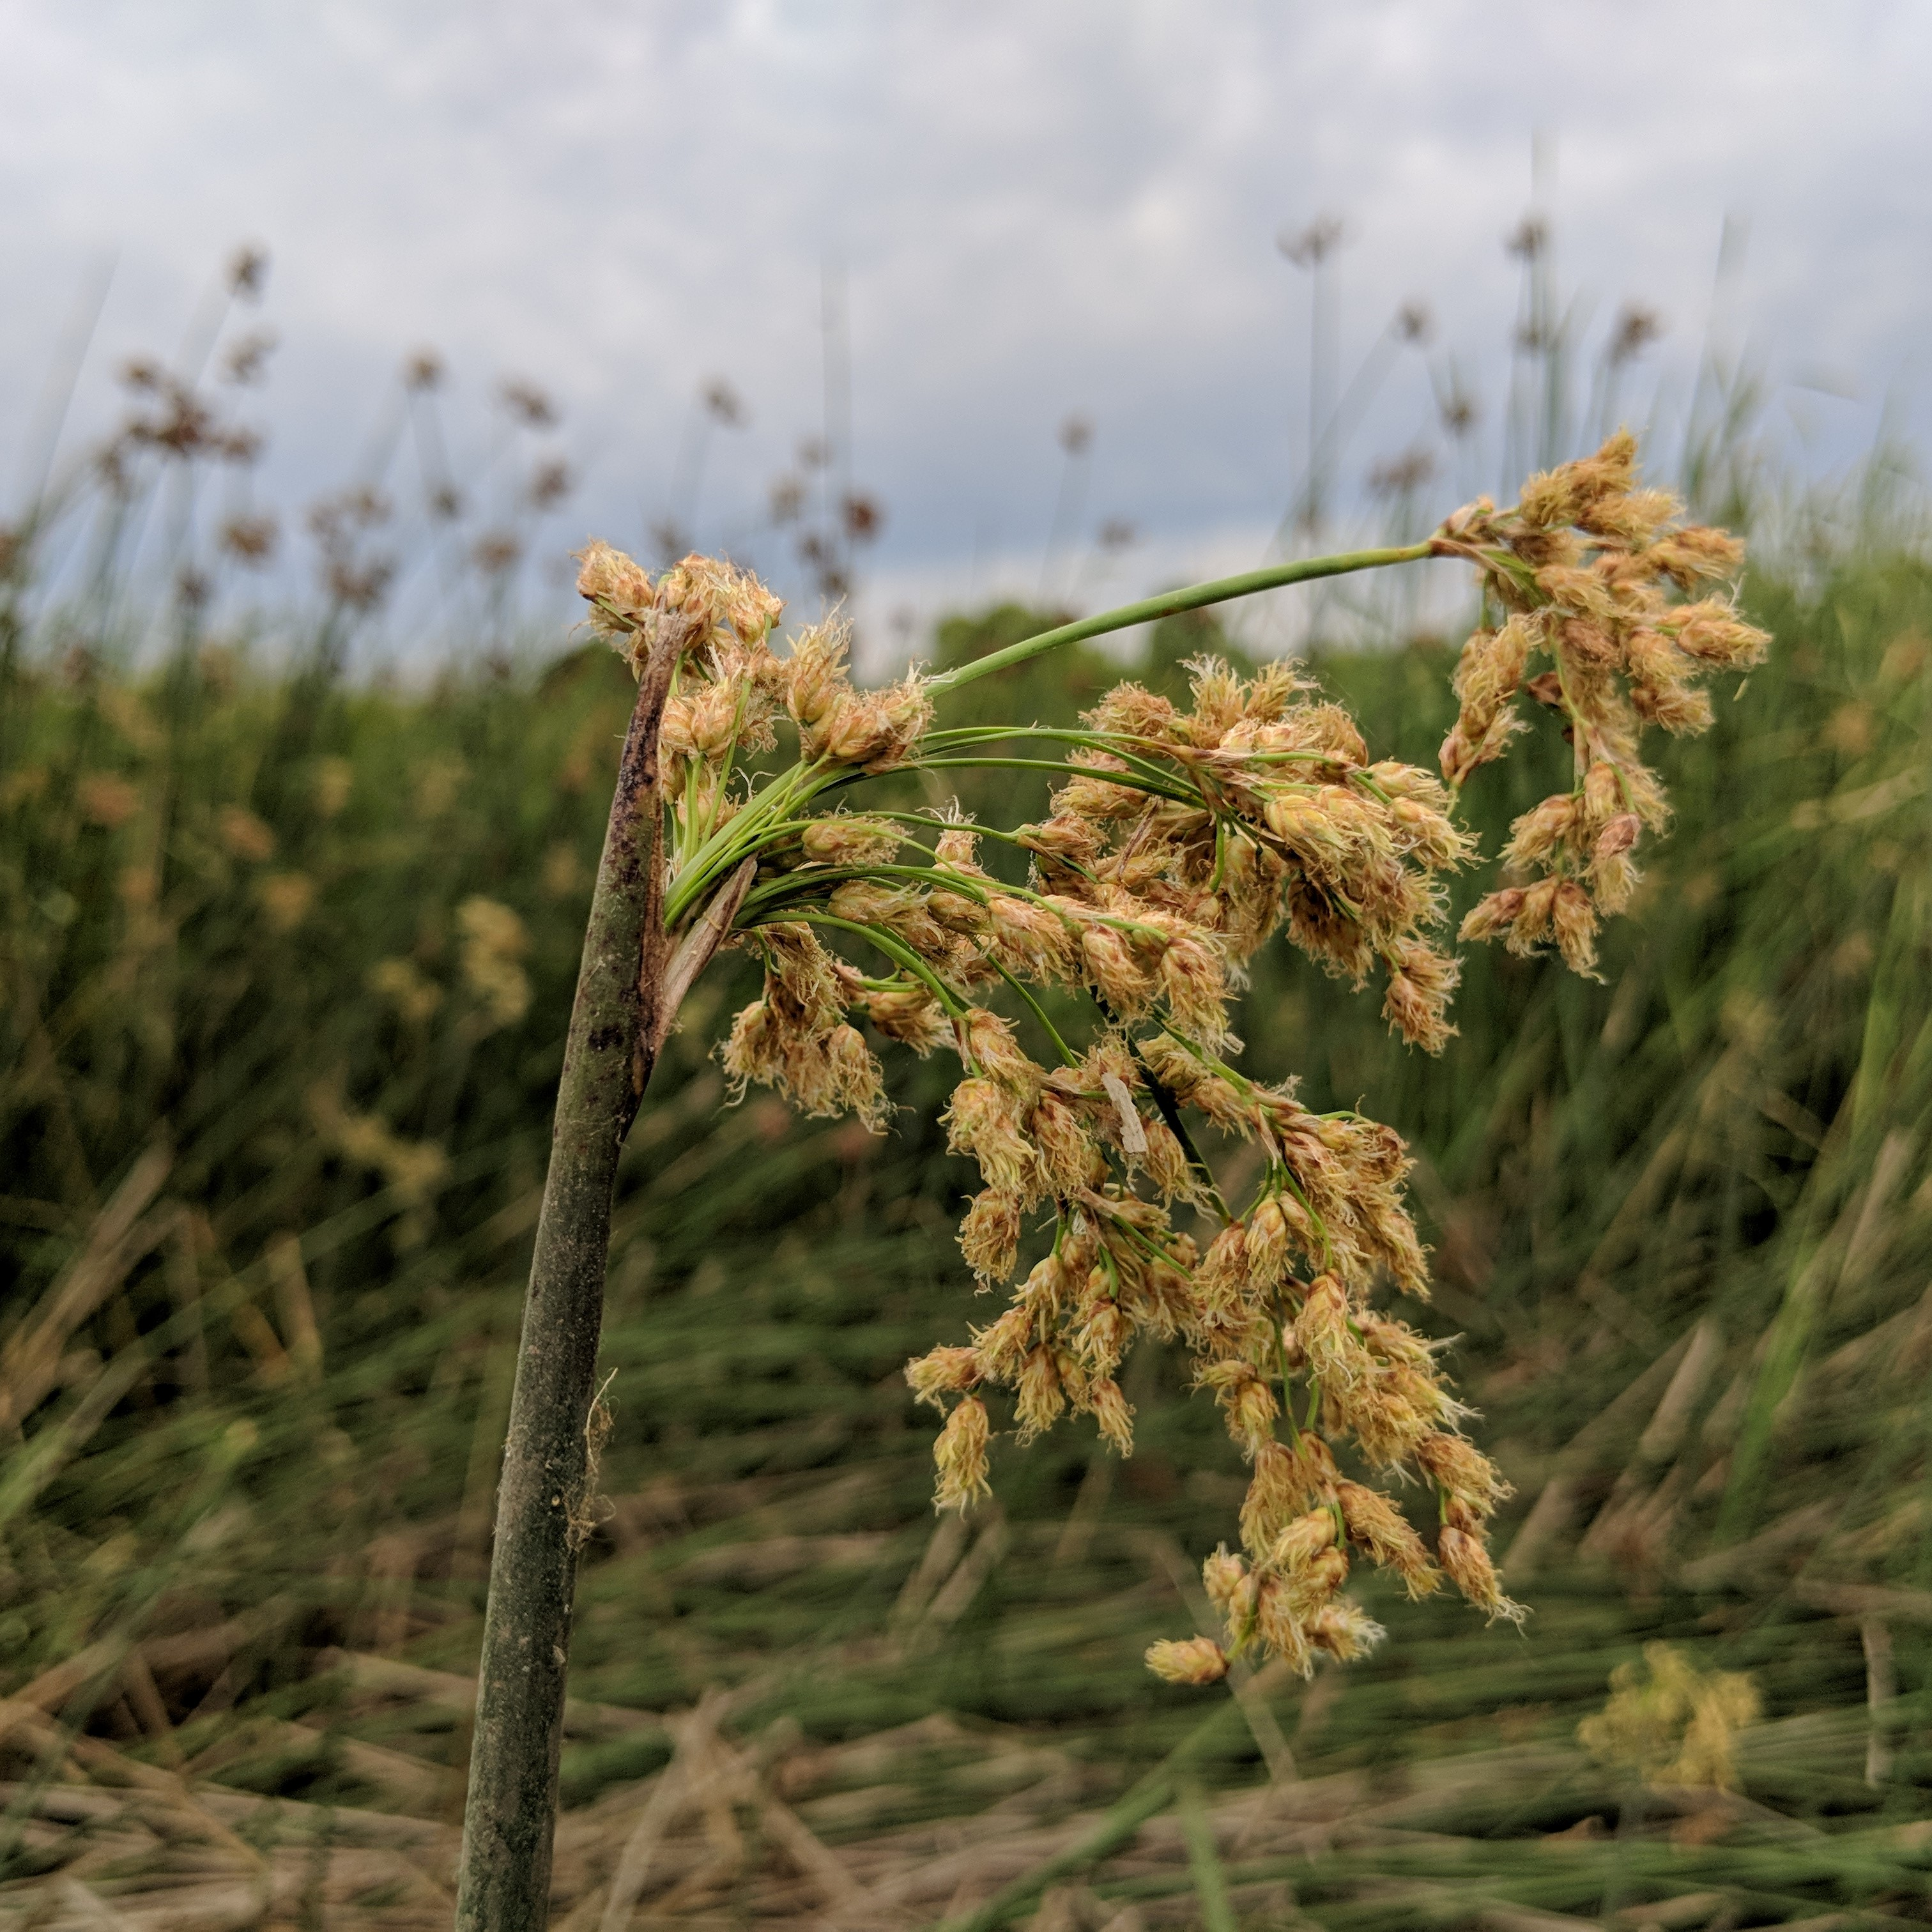
\includegraphics[width=0.5\linewidth]{../_chapter_materials/bulrush} 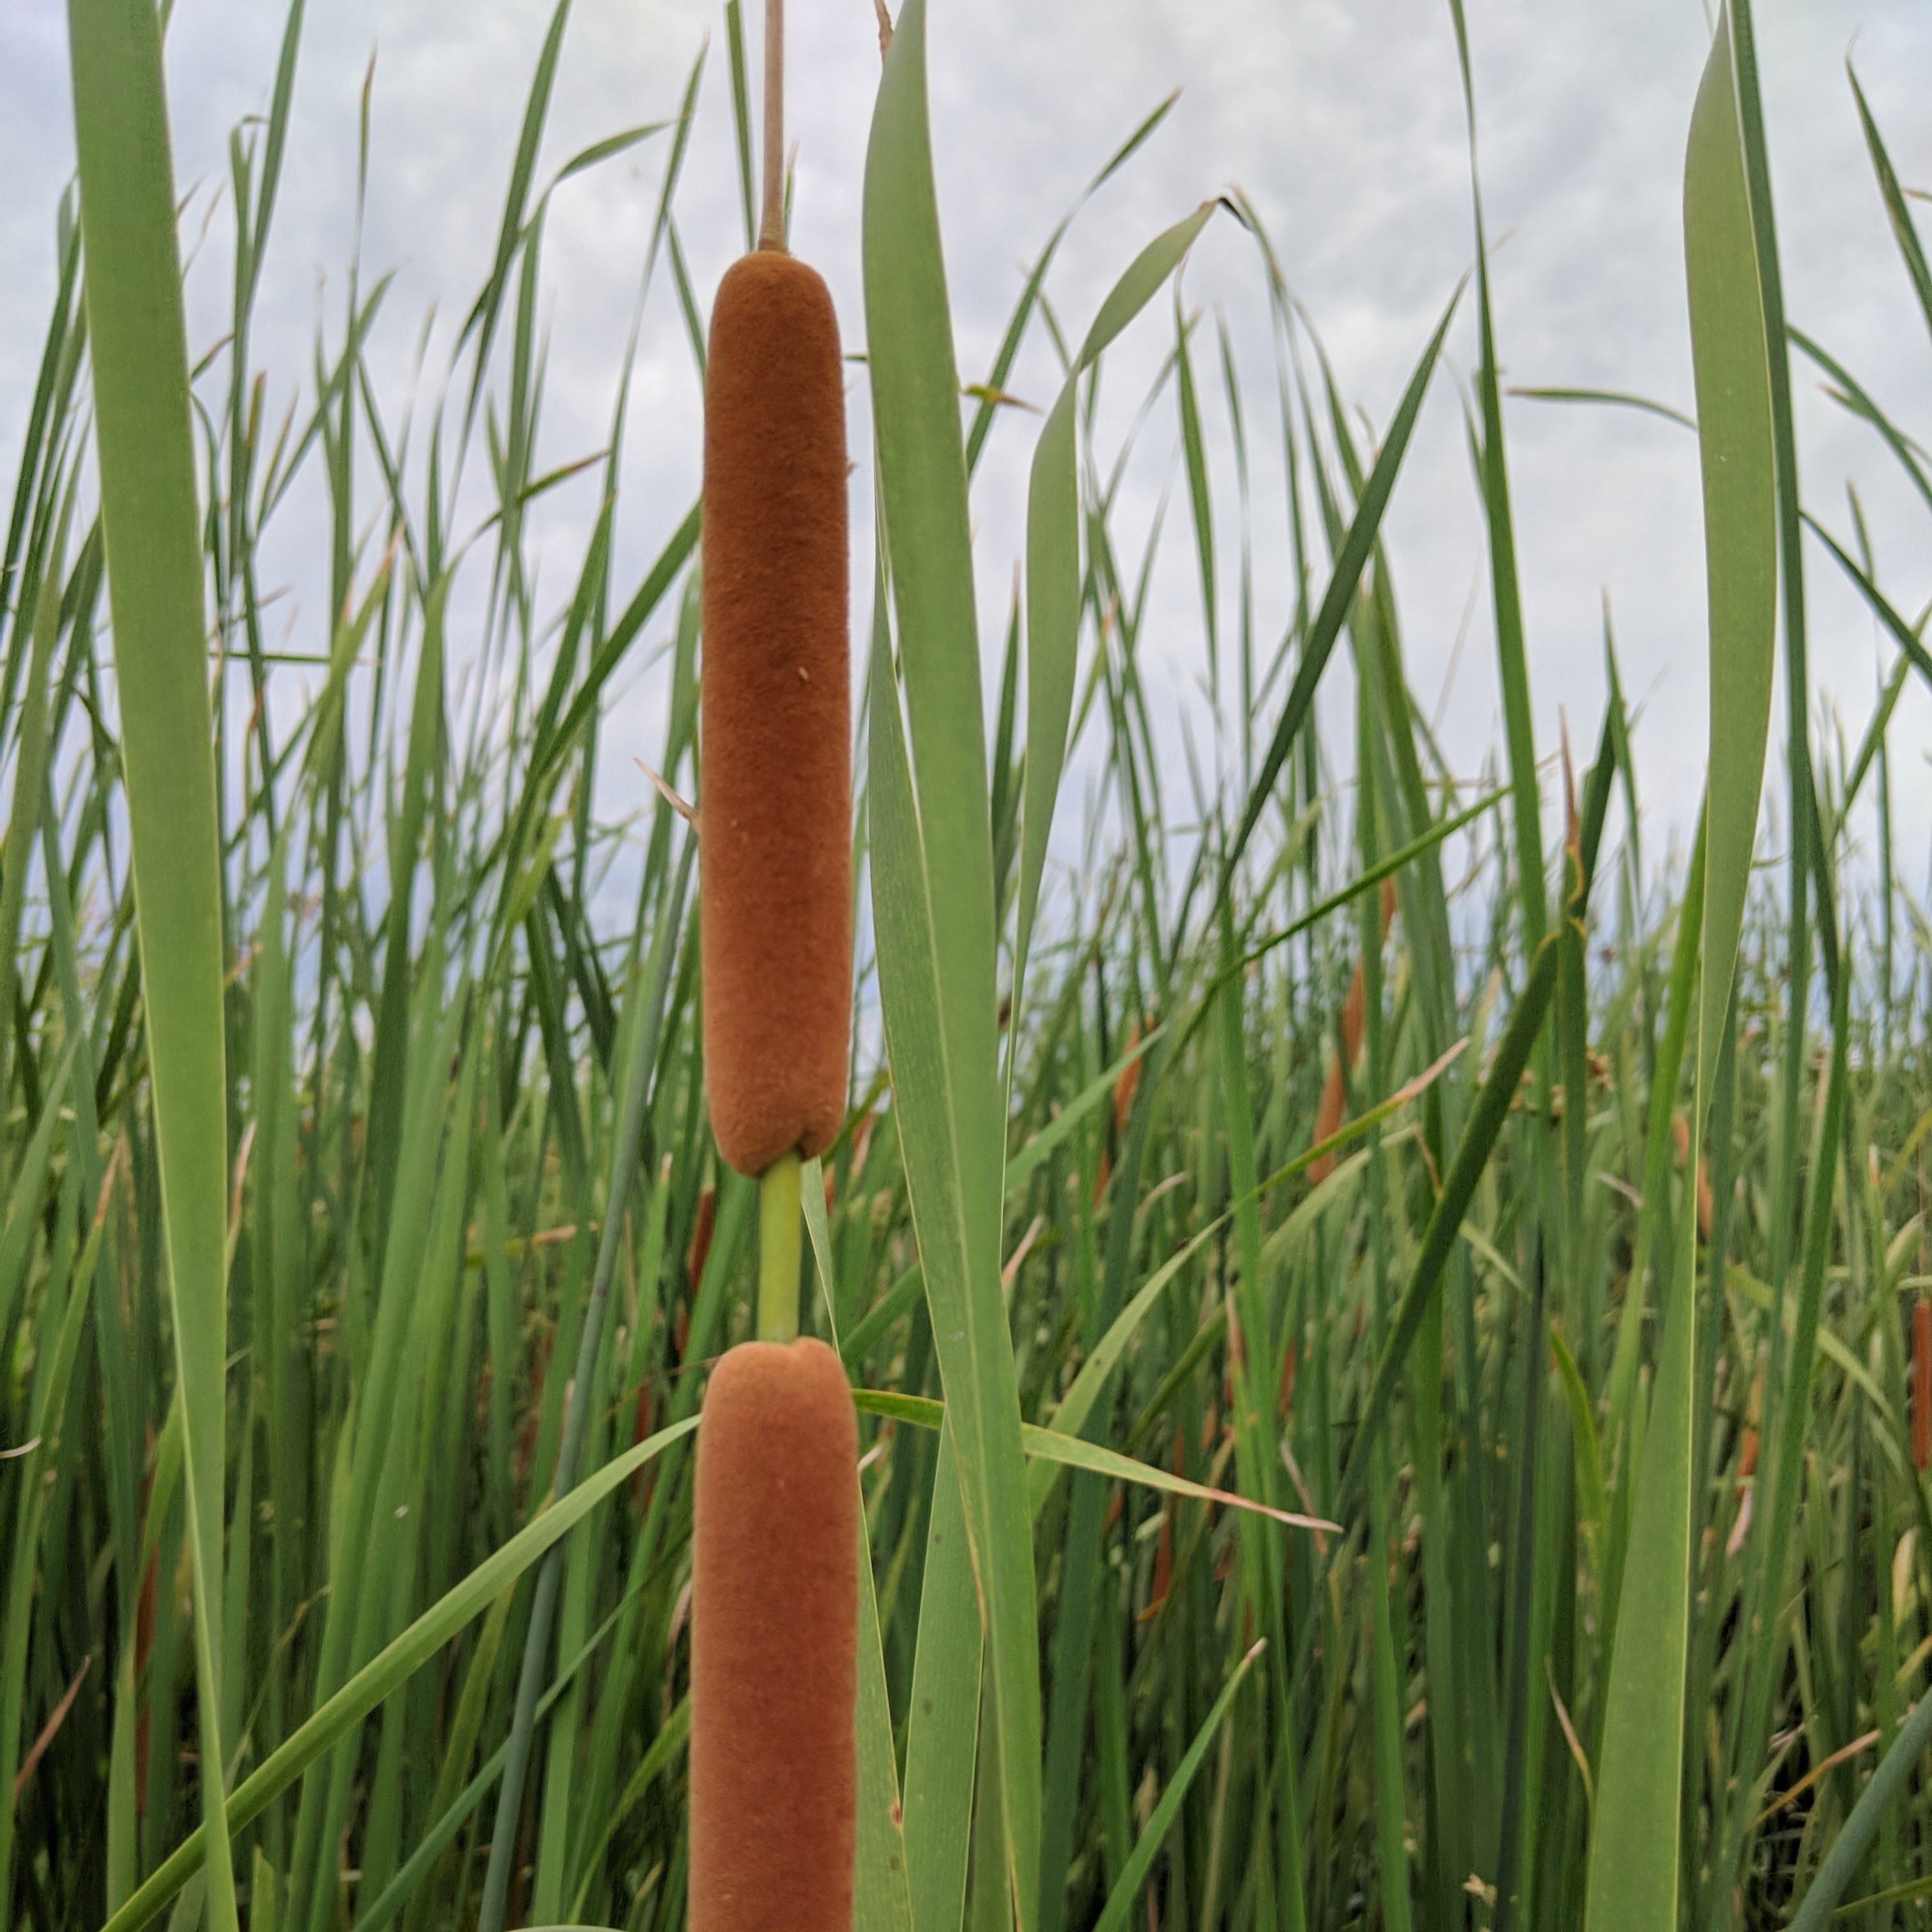
\includegraphics[width=0.5\linewidth]{../_chapter_materials/cattail} \caption{Bulrush (\textit{Schenoplectus}, left panel) and cattail (\textit{Typha}, right panel) are two common wetland plants that compete for similar resources. Bulrush are characterized by round stems and an inflorescence (i.e. flower) that emerges from the side of the stem, while cattail have semi-circular leaves and a large, cylindrical infloresence.}\label{fig:organisms}
\end{figure}

\hypertarget{objectives}{%
\section{Objectives}\label{objectives}}

You will collect vegetation data from two zones in the LWWs which have
different management histories (Fig. 2). One area in Cell 1 adjacent to
the floating boardwalk is a high visitation area where frequent
management has taken place. In contrast, Cell 2 has had virtually no
management. Five transects will be made originating in Cell 1, and five
in Cell 2. Data about community composition will be recorded from 5
quadrats (area of 1 m\textsuperscript{2}) along each transect.

\begin{figure}
\centering
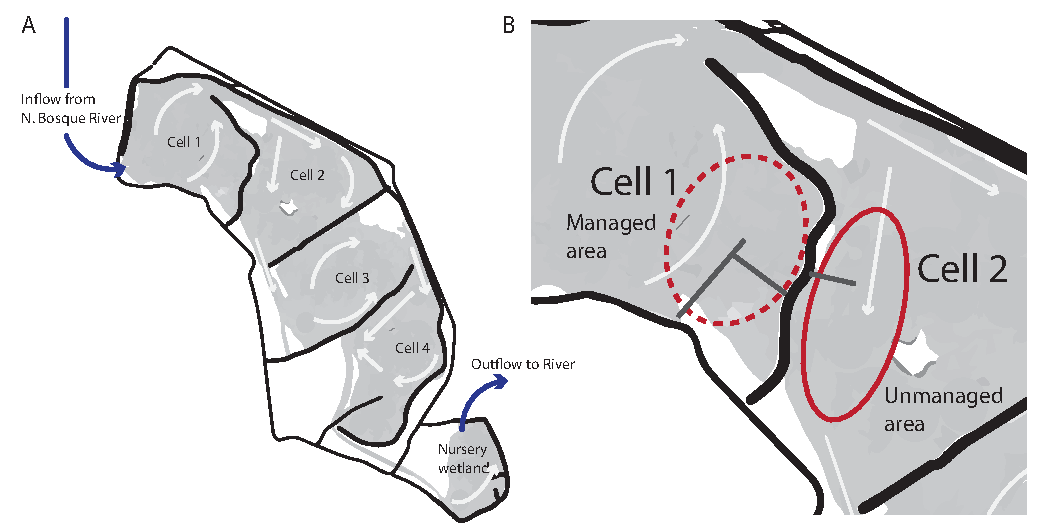
\includegraphics{../_chapter_materials/lww_figure.pdf}
\caption{The Lake Waco Wetlands (LWW), near Waco Tx. (A) Water flows
from the wetland inflow at the head of Cell 1 to the outflow after the
nursery wetlands. (B) Cell 1 is managed by LWW staff, while Cell 2 is
unmanaged.}
\end{figure}

\hypertarget{materials-methods}{%
\section{Materials \& methods}\label{materials-methods}}

\hypertarget{materials}{%
\subsection{Materials}\label{materials}}

\begin{multicols}{2}
\begin{itemize}{}
  \item Quadrat (m\textsuperscript{2})
  \item Depth pole
  \item Transect tape
  \item Field datasheet and clipboard
\end{itemize}
\end{multicols}

\hypertarget{methods}{%
\subsection{Methods}\label{methods}}

In each area sampled, place 5 quadrats along 5 parallel transects. These
will originate from the either the boardwalk or the levee between cells.
Place quadrats approximately 10 m apart. In each quadrat, record the
depth (in cm), rank \% cover, the presence of cattail and bulrush, and
if cattail or bulrush is the dominant species. If another species is
dominant, generate a descriptive `common name' that we may later use to
identify the plant. Also record the species richness of each quadrat.

\hypertarget{data-analysis}{%
\subsection{Data analysis}\label{data-analysis}}

Using the data generated and appropriate statistical analyses
(contingency table or t-test), address the following questions:

\begin{enumerate}
\def\labelenumi{\arabic{enumi}.}
\tightlist
\item
  Is management activity influencing the \textbf{abundance} of cattail?

  \begin{itemize}
  \tightlist
  \item
    A 2x2 contingency table is appropriate for this question.
  \end{itemize}
\item
  Is management activity influencing the \textbf{dominance} of cattail?

  \begin{itemize}
  \tightlist
  \item
    A 2x2 contingency table is appropriate for this question.
  \end{itemize}
\item
  Is management activity influencing \textbf{species richness}?

  \begin{itemize}
  \tightlist
  \item
    Most suited to a t-test, but could also be address using a 2x2
    contingency table.
  \end{itemize}
\item
  Does cattail dominance influence \textbf{species richness}?

  \begin{itemize}
  \tightlist
  \item
    Most suited to a t-test, but could also be address using a 2x2
    contingency table. For this question, the grouping variable is
    \emph{cattail dominance}, so you should use data from both cells!
  \end{itemize}
\end{enumerate}

\pagebreak

\hypertarget{lab-report-specifics}{%
\section{Lab report specifics}\label{lab-report-specifics}}

\begin{enumerate}
\def\labelenumi{\arabic{enumi}.}
\tightlist
\item
  Introduction

  \begin{itemize}
  \tightlist
  \item
    Why manage ecosystems?
  \item
    Why sample vegetation?
  \item
    Objectives
  \item
    Hypotheses
  \end{itemize}
\item
  Methods

  \begin{itemize}
  \tightlist
  \item
    Experimental design
  \item
    Review how data was collected
  \item
    Calculations / statistics
  \end{itemize}
\item
  Results

  \begin{itemize}
  \tightlist
  \item
    Question 1 (text \textbf{AND} graph/table)
  \item
    Question 2 (text \textbf{AND} graph/table)
  \item
    Question 3 (text \textbf{AND} graph/table)
  \item
    Question 4 (text \textbf{AND} graph/table)
  \end{itemize}
\item
  Discussion

  \begin{itemize}
  \tightlist
  \item
    Hypotheses rejected/supported
  \item
    Provide a coherent explanation/interpretation of your results
  \end{itemize}
\end{enumerate}




\newpage
\singlespacing 
\end{document}
